\section{Discriminator and Generator
implementation}\label{discriminator-and-generator-implementation}

In this notebook, you will implement the generator and discriminator
models. These models will be use in the last exercise of this lesson to
train your first GAN network!

\subsection{Discriminator}\label{discriminator}

The discriminator network is going to be a pretty typical linear
classifier. To make this network a universal function approximator,
we'll need at least one hidden layer, and these hidden layers should
have one key attribute: \textgreater{} All hidden layers will have a
\href{https://pytorch.org/docs/stable/nn.html\#torch.nn.LeakyReLU}{Leaky ReLu} activation function applied to their outputs.

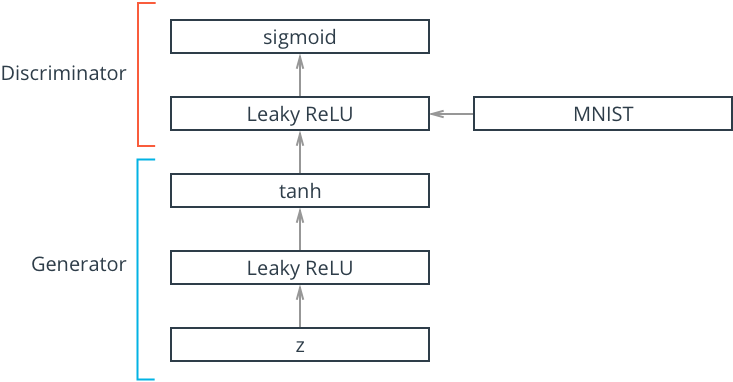
\includegraphics[width=0.5\linewidth]{img//genAdvNet//gan/gan_network.png}

\paragraph{Leaky ReLu}\label{leaky-relu}

We should use a leaky ReLU to allow gradients to flow backwards through
the layer unimpeded. A leaky ReLU is like a normal ReLU, except that
there is a small non-zero output for negative input values.

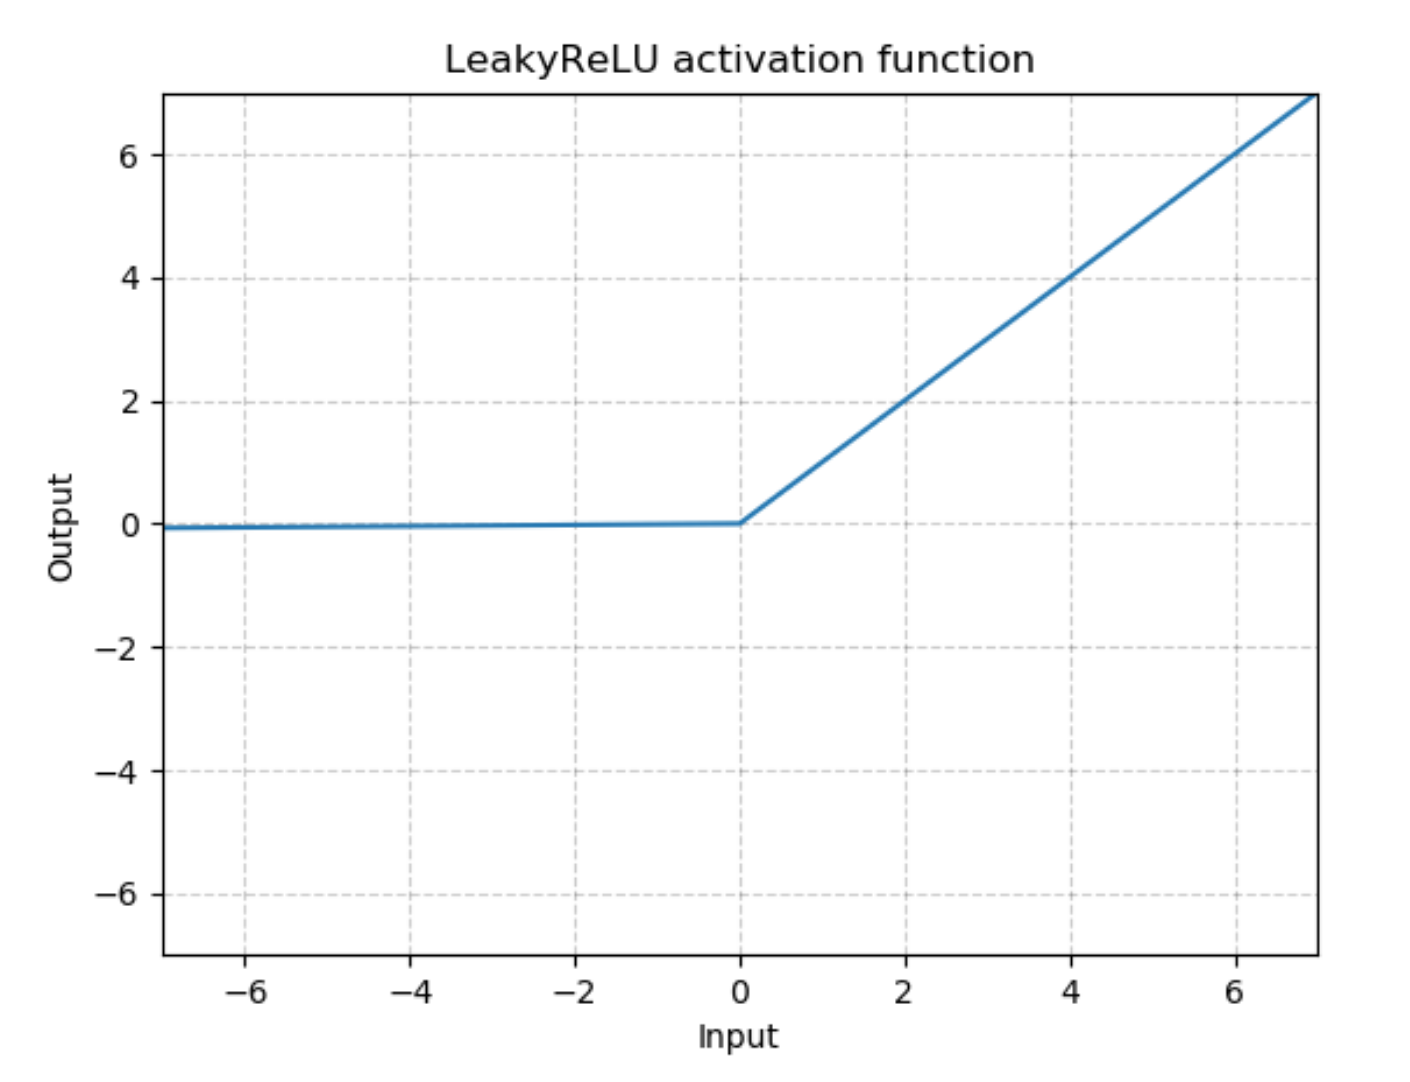
\includegraphics[width=0.5\linewidth]{img//genAdvNet//gan/leaky_relu.png}

\paragraph{Output}\label{output}

We'll also take the approach of using a more numerically stable loss
function on the outputs. Recall that we want the discriminator to output
a value 0-1 indicating whether an image is \emph{real or fake}.
\textgreater{} We will ultimately use
\href{https://pytorch.org/docs/stable/nn.html\#bcewithlogitsloss}{BCEWithLogitsLoss},
which combines a \lstinline{sigmoid} activation function
\textbf{and} binary cross entropy loss in one function.

So, our final output layer should not have any activation function
applied to it.

\paragraph{Structure}\label{structure}

The discriminator takes a high dimensional input (for example, an image)
and outputs a single score value. Linear layers in the discriminator
should have a number of neurons such that the dimensions of their output
is smaller than the dimension of their input.

\subsubsection{First exercise}\label{first-exercise}

Implement a discriminator network. Your network should: 
\begin{itemize}
    \item use fully connected layer and leaky relu
    \item output a single logit
    \item take a image asinput
\end{itemize}
\begin{lstlisting}[language=Python]
import torch
import torch.nn as nn

import tests
\end{lstlisting}

\begin{lstlisting}[language=Python]
class Discriminator(nn.Module):
    """
    Discriminator model:
    args: 
    - input_dim: dimension of the input data. For example, for a 28 by 28 grayscale image, the input size is 784
    - hidden_dim: a parameter that controls the dimensions of the hidden layers. 
    """
    def __init__(self, input_dim: int, hidden_dim: int):
        super(Discriminator, self).__init__()
        self.model = nn.Sequential(
            # Flatten image
            nn.Flatten(),
            # Hidden layers, activations & dropout
            nn.Linear(input_dim, hidden_dim),
            nn.LeakyReLU(0.1),
            nn.Dropout(0.2),
            nn.Linear(hidden_dim, hidden_dim // 2),
            nn.LeakyReLU(0.1),
            nn.Dropout(0.2),
            nn.Linear(hidden_dim // 2, hidden_dim // 4),
            nn.LeakyReLU(0.1),
            nn.Dropout(0.2),
            nn.Linear(hidden_dim // 4, 1)
        )
        #### 
        # IMPLEMENT HERE
        ####
        
    def forward(self, x: torch.Tensor) -> torch.Tensor:
        #### 
        # IMPLEMENT HERE
        ####
        return self.model(x)
\end{lstlisting}

\begin{lstlisting}[language=Python]
# for a 28x28 grayscale image flattened, the input dim is 784
input_dim = 784
hidden_dim = 256

discriminator = Discriminator(input_dim, hidden_dim)
tests.check_discriminator(discriminator, input_dim)
\end{lstlisting}

\begin{lstlisting}
Congrats, you successfully implemented your discriminator
\end{lstlisting}

\subsection{Generator}\label{generator}

The generator network will be almost exactly the same as the
discriminator network, except that we're applying a
\href{https://pytorch.org/docs/stable/nn.html\#tanh}{tanh activation
function} to our output layer.

\paragraph{tanh Output}\label{tanh-output}

The generator has been found to perform the best with \(tanh\) for the
generator output, which scales the output to be between -1 and 1,
instead of 0 and 1.

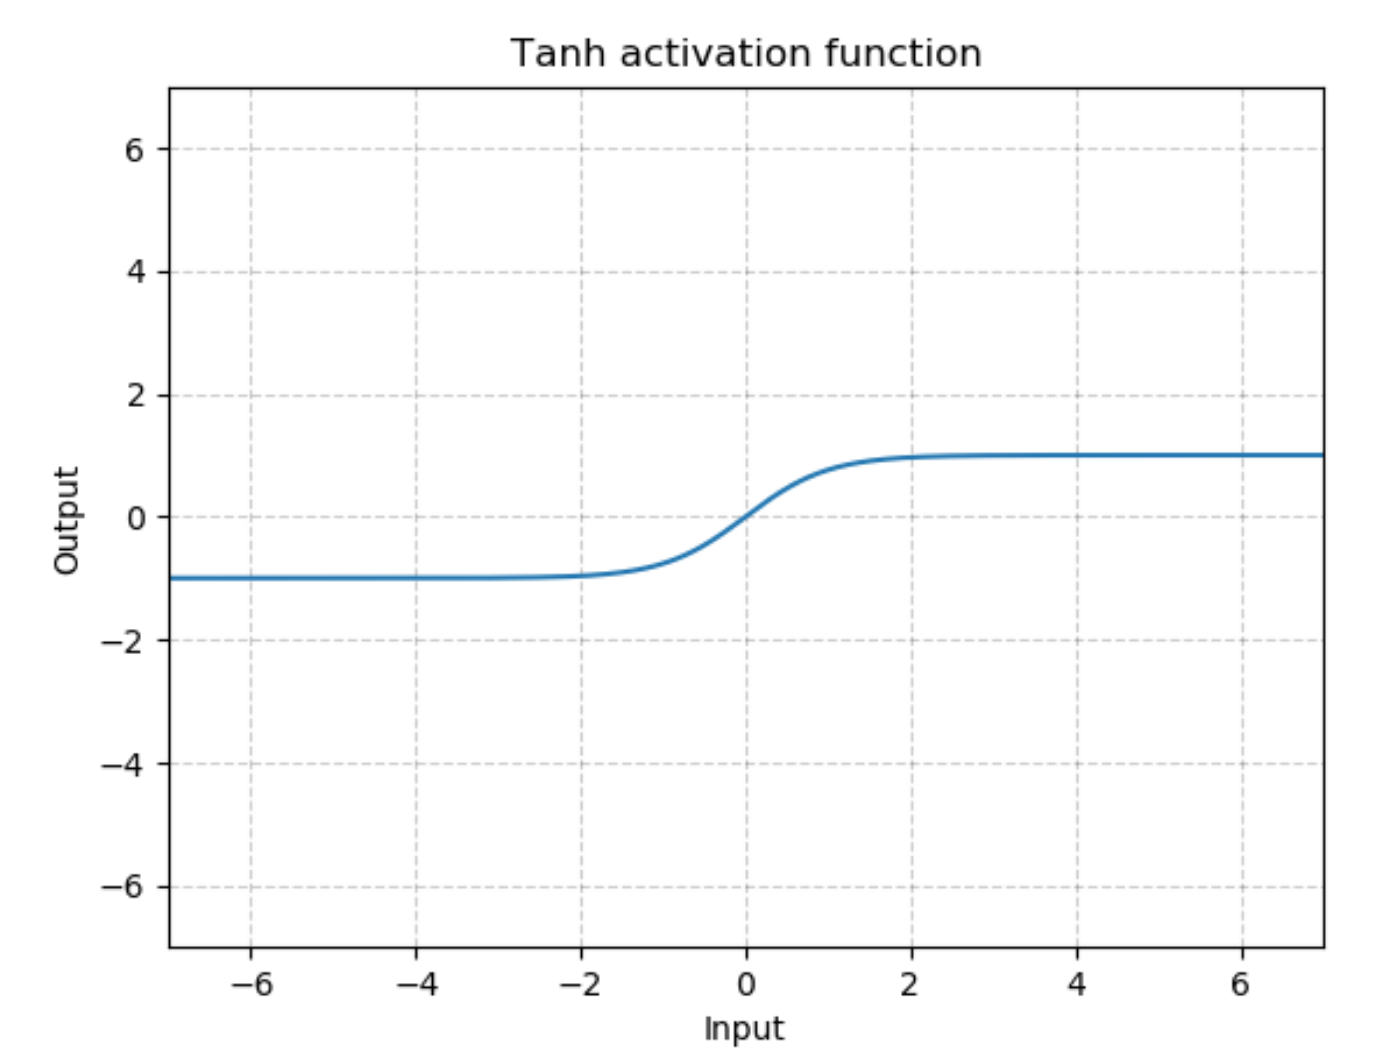
\includegraphics[width=0.5\linewidth]{img//genAdvNet//gan/tanh_fn.png}

Recall that we also want these outputs to be comparable to the
\emph{real} input pixel values, which are read in as normalized values
between 0 and 1. \textgreater{} So, we'll also have to \textbf{scale our
real input images to have pixel values between -1 and 1} when we train
the discriminator.

\subsection{Second Exercise}\label{second-exercise}

Implement a generator network. Your network should: * use fully
connected, leaky relu and tanh layers * take a latent as input * output
a vector (we will later reshape it as an image)

\begin{lstlisting}[language=Python]
class Generator(nn.Module):
    def __init__(self, latent_dim: int, hidden_dim: int, output_size: int):
        super(Generator, self).__init__()
        self.model = nn.Sequential(
            # Hidden layers, activations & dropout
            nn.Linear(latent_dim, hidden_dim),
            nn.LeakyReLU(0.1),
            nn.Dropout(0.2),
            nn.Linear(hidden_dim, hidden_dim * 2),
            nn.LeakyReLU(0.1),
            nn.Dropout(0.2),
            nn.Linear(hidden_dim * 2, hidden_dim * 4),
            nn.LeakyReLU(0.1),
            nn.Dropout(0.2),
            # Final layer
            nn.Linear(hidden_dim * 4, output_size),
            # Final tanh function to output layer
            nn.Tanh()
        )
        #### 
        # IMPLEMENT HERE
        ####

    def forward(self, x: torch.Tensor) -> torch.Tensor:
        #### 
        # IMPLEMENT HERE
        ####
        return self.model(x)
\end{lstlisting}

\begin{lstlisting}[language=Python]
latent_dim = 128
hidden_dim = 256
output_dim = 784

generator = Generator(latent_dim, hidden_dim, output_dim)
tests.check_generator(generator, latent_dim, output_dim)
\end{lstlisting}

\begin{lstlisting}
Congrats, you successfully implemented your generator
\end{lstlisting}
